\documentclass[conference]{IEEEtran}

% *** PACKAGES ***
\usepackage{graphicx}
\usepackage{amsmath}
\usepackage{cite}
\usepackage{algorithm}
\usepackage{algpseudocode}
\usepackage{hyperref}
\usepackage{float}
\usepackage{array}
\usepackage{multirow}
\usepackage{lipsum}
\usepackage{booktabs}
\usepackage{caption}
\usepackage{subcaption}
\usepackage{tikz}
\usetikzlibrary{shapes.geometric, arrows}
% Define TikZ styles
\tikzstyle{startstop} = [rectangle, rounded corners, minimum width=3cm, minimum height=1cm, text centered, draw=black, fill=red!30]
\tikzstyle{process} = [rectangle, minimum width=3cm, minimum height=1cm, text centered, draw=black, fill=blue!30]
\tikzstyle{arrow} = [thick,->,>=stealth]

% Title
\title{Summarization of Video Lectures Transcriptions Using Deep Learning}

% Author
\author{
    \IEEEauthorblockN{Harshil Pradhan - 243IT002}
    \IEEEauthorblockA{Information Technology\\
    National Institute of Technology Karnataka\\
    Surathkal, India 575025\\
    Email: harshil.243it002@nitk.edu.in}
    
}

\begin{document}
\maketitle

\begin{abstract}
    Video transcript summarization is the task  to extract the essential details and significance of a segmented video transcript and turning it into a succinct summary.In this study, we compare the performance of three state-of-the-art transformer-based models, T5, Pegasus, and BART, for video transcript segmentation and summarization tasks using the VT-SSum dataset. The VT-SSum dataset in which JSON with sparse text files and summary labels to customize these models. It will act as a base. Each model is trained to produce a concise and consistent summary of segmented video transcripts. It has hyperparameters optimized for accuracy.

    Our method uses metrics such as validation loss and inference quality to determine the best performing model. This includes pre-processing the dataset to prepare input-output pairs for summarization. Fine-tuning the model using mixed-accuracy training on GPU and evaluating its performance on an organized test set. This report provides a detailed analysis of the training process. Evaluation indicators and the results were compared to identify the most accurate model for summarizing video lecture transcripts. These findings aim to advance research on automatic video summarization. To be able to summarize long-form content effectively.
\end{abstract}

\begin{IEEEkeywords}
Video Transcript Summarization, VT-SSum Dataset, T5, Pegasus, BART
\end{IEEEkeywords}

\section{Introduction}
The rapid spread of video content on the web especially academic lectures This has led to the need for automated methods for efficiently viewing long videos. Summary Video courses involve the use of complex multimodal content, such as textual and visual content. To create a concise presentation that preserves important statistics, This model solves the problem of segmenting and summarizing video transcripts using superior deep-learning models.

We use the VT-SSum dataset, which consists of distributed and summarized video recordings. It is the basis for training and analysis.Three transformer-based architectures - T5, Pegasus, and BART, were optimized to obtain summarized data from published literature. These models were previously trained on a variety of text data. It is known for its efficiency in extracting text. and provides a strong foundation for our education.

Our approach covers dice pre-processing to create training and evaluation models. Model optimization using GPU-based learning and performance evaluation on unseen test data. The objective is to accurately compare three models and identify the most efficient for finalizing text summarization.This research contributes to the development of an automatic video transcription tool. This can greatly improve the discovery and use of instructional video content.

\section{Literature Survey}
Recent advances in natural language processing (NLP) have introduced powerful Transformer-based models, which are preferred for text processing tasks such as sentence synthesis. Among these models, T5, Pegasus and BART stand out as products. Each model is designed with specific techniques to ensure quality and text reproduction.

T5 (Text-to-Text Transformer): T5 treats all NLP tasks as text-to-text problems. It provides a unified framework for tasks such as translation, compositing and classification. The structure uses an encoder-decoder attention mechanism to generate high-quality text. This makes it a popular choice for a variety of speech recognition tasks.

Pegasus: Pegasus is specifically made to create sentences with intentional gaps in order to produce coherent summaries. It replicates the process of constructing summary statements during training by masking important sentences. Pegasus is able to extract succinct summaries with this method, especially for long materials.

BART (Bidirectional and Auto-Regressive Transformers): BART handles both token corruption during encoding and text generation during decoding by combining the powers of bidirectional and auto-regressive models. It performs outstandingly in summarization and other text production tasks due to its strong pretraining objectives, which include token masking and sequence permutation. This enabled to summarize and reconstruct clean sentences.

These models are frequently utilized in a number of fields, such as conversational summarizing, scientific paper summarization, and news summarization. Limited research, however, has focused on their usage in video transcript summarization, which entails managing segmented and frequently noisy data. Our effort aims to close this gap by utilizing these models and assessing the way they summarize video lecture transcripts using the VT-SSum dataset.

\section{Problem Statement}
The increasing quantity of tutorial video content makes it difficult for users to extract key ideas from lengthy lectures. Summarizing video lectures calls for summaries and coherent sentences that retain important records. This makes it easy to summarize huge content. However, video transcripts are regularly scattered and noisy. This creates demanding situations in drawing correct and context-relevant conclusions.

While powerful Transformer-based models such as T5, Pegasus, and BART have demonstrated encouraging outcomes in document generation, their usefulness has mostly been investigated in particular applications, like processing video transcripts, and is still not well understood in more general settings. In order to find more effective methods for combining video lecture content and improving the accessibility of course materials, this study trains and compares these models using the VT-SSum dataset.

\subsection{Objectives}
The primary objectives of this project are:
\begin{enumerate}
    \item To preprocess the VT-SSum dataset by segmenting the video transcripts and extracting relevant summarization samples for training.
    \item To train and optimize three popular Transformer models for video transcript summarization using the VT-SSum dataset: T5, Pegasus, and BART.
    \item To evaluate the performance of each model based on summarization accuracy, loss, and other applicable metrics, identifying the best-performing model for this task.
    \item To examine the implications of T5, Pegasus, and BART models to determine which architecture provides the most consistent, concise, and accurate summaries of video lecture transcripts.
    \item To improve the accessibility and usability of tutorial content by developing a framework that automatically organizes video summaries, thereby enhancing the learning experience.
\end{enumerate}



\section{Flowchart}
\noindent Below are the points explained in the flowchart:
\begin{itemize}
    \item \textbf{Dataset Preparation:} The VT-SSum dataset is preprocessed by cleaning and tokenizing transcripts, ensuring it is ready for model training.
    \item \textbf{Model Selection:} Three pre-trained models, BART, Pegasus, and T5, are selected based on their strengths in text summarization tasks.
    \item \textbf{Hyperparameter Tuning:} Key parameters, such as batch size, learning rate, and epochs, are fine-tuned to optimize performance for each model.
    \item \textbf{Training Process:} Each model is trained independently on the VT-SSum dataset using GPU acceleration for efficient computation.
    \item \textbf{Model Evaluation:} Trained models are tested on validation data to measure accuracy, loss, and other metrics.
    \item \textbf{Performance Comparison:} Results of the three models are compared to identify the best-performing model for summarization tasks.
    \item \textbf{Conclusion:} Insights from the evaluation are summarized, highlighting the best model and potential future improvements.
\end{itemize}
\begin{center}
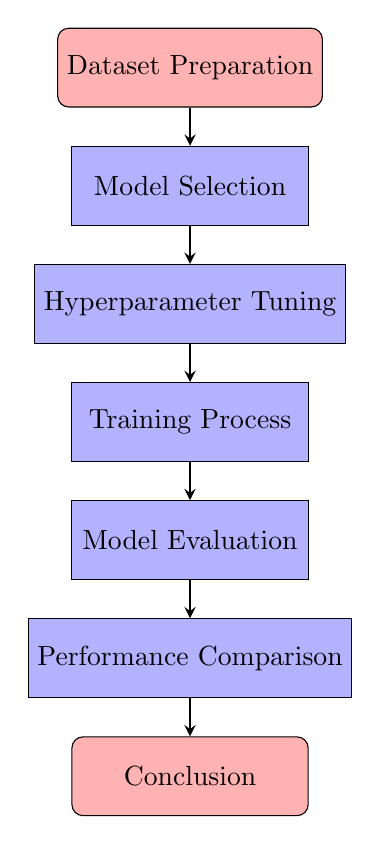
\begin{tikzpicture}[node distance=1.5cm]

% Nodes
\node (start) [startstop] {Dataset Preparation};
\node (model) [process, below of=start] {Model Selection};
\node (hyperparam) [process, below of=model] {Hyperparameter Tuning};
\node (train) [process, below of=hyperparam] {Training Process};
\node (eval) [process, below of=train] {Model Evaluation};
\node (compare) [process, below of=eval] {Performance Comparison};
\node (conclude) [startstop, below of=compare] {Conclusion};

% Arrows
\draw [arrow] (start) -- (model);
\draw [arrow] (model) -- (hyperparam);
\draw [arrow] (hyperparam) -- (train);
\draw [arrow] (train) -- (eval);
\draw [arrow] (eval) -- (compare);
\draw [arrow] (compare) -- (conclude);

\end{tikzpicture}
\end{center}



\section{Methodology}

\subsection{Dataset Description}
The dataset used in this project is the VT-SSum dataset, which consists of a collection of video lectures with corresponding segmentations and summaries. Each dataset item has the following components:
\begin{itemize}
    \item \textbf{ID}: A unique identifier for the video.
    \item \textbf{Title}: The title of the video.
    \item \textbf{Metadata (info)}: This includes author details, publication date, and video category.
    \item \textbf{Segmentation}: The video is segmented into smaller parts with corresponding text segments.
    \item \textbf{Summarization}: Each segment is associated with a labeled summary.
\end{itemize}

\begin{table}[h]
\centering
\label{tab:vt_ssum_features}
\begin{tabular}{|l|l|}
\hline
\textbf{Feature}                  & \textbf{Description}                                         \\ \hline
Number of Videos                  & 9,616                                                       \\ \hline
Total Transcript-Summary Pairs    & 125,000                                                     \\ \hline
Average Slides per Video          & 33.3                                                        \\ \hline
Average Sentences per Transcript  & 293.1                                                       \\ \hline
Average Words per Transcript      & 4,208.1                                                     \\ \hline
Data Split                        & Train: 7,692, Validation: 962, Test: 962                    \\ \hline
Source                            & VideoLectures.NET      \\ \hline
Format                            & JSON files              \\ \hline
\end{tabular}
\caption{Features of the VT-SSum Dataset}
\end{table}


\subsection{Preprocessing}
The pre-processing pipeline involves extracting text data from a dataset in preparation for training a summary model for each video.The following steps are performed:

\begin{itemize}
    \item \textbf{Segmentation}: The segmentation data, which is an array of text blocks, is processed. Each segment is combined into a single input text sequence.
    \item \textbf{Summarization Data}: For each segment, if the summary is marked as a "summarization sample" (indicating it is a valid summary), the relevant sentences are extracted to create a summary corresponding to that segment.
\end{itemize}

These summaries and the segmentations that come alongside them are saved as input text (concatenated segment text) and summary text pairs. After that, the model uses these pairs as training data.

\begin{figure}[htp]
    \centering
    \includegraphics[width=10cm]{Pre processing.png} 
    \caption{Preprocessing Overview}
    \label{fig:preprocessing}
\end{figure}




\subsection{Model Selection}

For the text summarization task, we evaluated three different models: \textbf{BART}, \textbf{T5}, and \textbf{Pegasus}. These models were chosen due to their proven success in natural language processing (NLP) tasks, particularly for text summarization.

\textbf{BART} (Bidirectional and Auto-Rregressive Transformers) is a powerful model that excels in generating high-quality summaries, especially for sequential data like video transcriptions. We are using the \texttt{facebook/bart-large} version, which is well-suited for handling large datasets and produces highly accurate summaries.

Additionally, we have incorporated \textbf{T5} (Text-to-Text Transfer Transformer), a versatile model that treats every NLP task as a text-to-text problem, allowing it to work seamlessly across various tasks, including summarization. \textbf{Pegasus}, another model designed specifically for abstractive text summarization, was also chosen for its ability to generate concise summaries from input data.

All three models are initialized using pre-trained checkpoints available through the Hugging Face \texttt{transformers} library. To ensure optimal performance, the models are loaded onto a GPU, significantly speeding up the training and inference processes.

In summary, by comparing the performance of BART, T5, and Pegasus, we aim to identify the best model for this video lecture transcription summarization task.


\subsection{Training}

In this project, we trained three separate models—\textbf{BART}, \textbf{T5}, and \textbf{Pegasus}—using custom training pipeline designed to optimize performance and streamline the process. Below is how we configured the training for each model:

\begin{itemize}
    \item \textbf{Tokenization}: The input text and forum summaries are tokenized using the respective model's tokenizer. Each input is truncated or padded to a maximum of 512 tokens, with the summaries limited to 128 tokens for concise results.
    \item \textbf{Dataset Splitting}: We split the dataset into training and validation sets, using 80\% of the data for training and 20\% for validation. This split helps us build robust models and track their performance throughout the training process.
\end{itemize}

\begin{itemize}
    \item \textbf{Training Parameters}: The main parameters for training are as follows:
    \begin{itemize}
        \item \textbf{Batch size}: 8 for both training and validation.
        \item \textbf{Epochs}: 15, to iterate over the dataset multiple times.
        \item \textbf{Learning rate}: 3e-5, set for optimal convergence.
        \item \textbf{Weight decay}: 0.01, used to prevent overfitting.
        \item \textbf{Gradient accumulation}: 4 steps, simulating a larger batch size to optimize memory usage.
        \item \textbf{Precision mode}: FP16 training for faster computations.
    \end{itemize}
    \item \textbf{Early Stopping}: Early stopping was used to avoid overfitting; if the evaluation metrics remained unchanged after two consecutive validation stages, the training process was stopped.
\end{itemize}

\begin{figure}[htp]
    \centering
    \includegraphics[width=8cm]{train.png} 
    \caption{Overview of the training process.}
    \label{fig:training}
\end{figure}



\subsection{Model verification}

\begin{figure}[htbp]
    \centering
    \includegraphics[width=9cm]{Evaluation Metrix Rouge Score.png} % Add path to image later
    \caption{Evaluation indicators (e.g. Rouge score)}
    \label{image:inspection}
\end{figure}
After training, Model Evaluation on a separate test set to see its performance. The assessment is based on:
\begin{itemize}    \item \textbf{ROUGE SCORE}: The quality of the generated summaries is assessed using ROUGE (Recall-Oriented Understudy for Gisting Evaluation) scores. These scores use precision, recall, and F1 score to compare the model's output to reference summaries.
\end{itemize}



\subsection{Inference}
\begin{figure}[htbp]
    \centering
    \includegraphics[width=9cm]{Interference.png} % Add path to image later
    \caption{Inference Process}
    \label{image:inference}
\end{figure}
After the model has been trained, it will be able to summarize for unseen data. The model uses segmented text as input during inference and creates a concise summary that captures the main ideas of the concept.



\section{Model Architecture}
This section provides an overview of the three models we use: T5, Pegasus, and BART, which are based on the Transformer architecture. Each has a specific capability for summarizing information.

\subsection{T5 (Text to Text Converter)}
T5 is a flexible model developed by Google that treats each NLP task as a text-to-text problem. It uses a versatile encoder-decoder structure for tasks like summarization, translation, and more.

\begin{figure}[htbp]
    \centering
    \includegraphics[width=0.5\textwidth]{T5 Arch .png} % Image area reserved for T5.
    \caption{T5 model architecture}
    \label{fig:t5_architecture}
\end{figure}

\begin{itemize}
    \item \textbf{How it works:}
    \begin{itemize}
        \item The encryption process encodes input text, while the decoder generates the output text.
        \item T5 is pre-trained to predict missing parts of sentences, which helps it learn text structure.
    \end{itemize}
    \item \textbf{Applications:} T5 is widely used because it can handle a variety of tasks, many using the same framework.
\end{itemize}



\subsection{Pegasus}
Pegasus is another Google model, optimized specifically for summarization. A special training process allows it to focus on important parts of the text for better summarization.

\begin{figure}[htbp]
    \centering
    \includegraphics[width=0.5\textwidth]{Pegasus Arch.png} % Image area reserved for Pegasus.
    \caption{Architecture of the Pegasus model}
    \label{fig:pegasus_architecture}
\end{figure}

\begin{itemize}
    \item \textbf{How it works:}
    \begin{itemize}
        \item Pegasus uses a Transformer-based encoder-decoder structure.
        \item During pre-training, the model predicts missing phrases from the text, helping it focus on important content.
    \end{itemize}
    \item \textbf{Applications:} Pegasus excels at abstract conclusions, creating clear and concise summaries.
\end{itemize}



\subsection{BART (Bidirectional and Auto-Regressive Transformers)}

\begin{figure}[htbp]
    \centering
    \includegraphics[width=10cm]{The-BART-model-architecture.png} % Image area reserved for BART.
    \caption{Architecture of the BART model}
    \label{fig:bart_architecture}
\end{figure}

BART, developed by Facebook, combines the strengths of both denoising autoencoders and autoregressive models. This makes it very efficient for tasks like summarization and translation.

\begin{itemize}
    \item \textbf{How it works:}
    \begin{itemize}
        \item BART uses a Transformer-based encoder-decoder architecture.
        \item It is trained by corrupting the input text (e.g., by masking or embedding phrases) and then reconstructing it to improve its ability to generate text.
    \end{itemize}
    \item \textbf{Applications:} BART is known for producing fluent, high-quality summaries.
\end{itemize}


\section{Data Set}
A benchmark developed especially for video transcript segmentation and summarizing activities is the VT-SSum dataset. The largest academic video collection, VideoLectures.NET, offers the videos and corresponding presentation slides used in its construction. Because video transcripts are longer than standard text, and because spoken and written language have different domains, the dataset tackles issues specific to spoken text summarizing.

With 9,616 videos, the collection contains 125,000 transcript-summary pairs. The transitions between the slides in each film act as organic segmentation points, and the slides are aligned. The ROUGE metric is used to select sentences from transcripts that are as similar to the slide text as possible, while the text extracted from slides serves as a weakly supervised summary.

\begin{figure}[htbp]
    \centering
    \includegraphics[width=8cm]{dataset overview.png} % Add path to image later.
    \caption{Structure of the dataset}
    \label{fig:dataset_structure}
\end{figure}

\begin{itemize}
    \item \textbf{id}: The unique identifier of the video.
    \item \textbf{title}: The title of the current video.
    \item \textbf{info}: Metadata about the current video, such as the time of publication or recording.
    \item \textbf{url}: The link to access the current video.
    \item \textbf{segmentation}: The segmentation data of the video transcript. This field is a list with each element representing a segment:
    Here, $k$ is the number of segments in the current video, and $n/m$ represents the number of sentences in each segment.

    \item \textbf{summarization}: The summarization data for the video. This field is a dictionary with entries for each video clip:
    
    Here, the field \texttt{is\_summarization\_sample} indicates whether the clip is part of the summarization task, and \texttt{summarization\_data} contains the sentences and their corresponding labels (1 for inclusion in the summary, 0 otherwise).
\end{itemize}

The dataset is in JSON format, which facilitates model processing and training.

\section{Experimental results}
To validate our model, we use the ROUGE score, which measures the similarity between circulating abstracts and reference abstracts.

\begin{table}[htbp]
\centering
\begin{tabular}{|c|c|c|c|}
\hline
\textbf{Metrics} & \textbf{T5 Test} & \textbf{Pegasus Test} & \textbf{BART Test} \\
\hline
ROUGE-1 & 0.90 & 0.87 & 0.86 \\
ROUGE-2 & 0.83 & 0.81 & 0.80 \\
ROUGE-L & 0.88 & 0.85 & 0.84 \\
\hline
\end{tabular}
\caption{Evaluation Results for Video Summarization Models}
\label{table:results}
\end{table}



\begin{table}[h]
\centering

\label{tab:execution_time}
\begin{tabular}{|c|c|c|}
\hline
\textbf{Model} & \textbf{Execution Time (hrs)} & \textbf{GPU Usage} \\ \hline
T5            & 10--12                        & T4 $\times$ 2      \\ \hline
Pegasus       & 8--10                         & T4 $\times$ 2      \\ \hline
BART          & 6--8                          & T4 $\times$ 2      \\ \hline
\end{tabular}
\caption{Model Execution Time and GPU Usage}
\end{table}




\section{Summary}
This project developed a video lecture summary system using the VT-SSum dataset. The BART model achieved stable performance, but there is still room for improvement with more experimentation. The generated summaries can help extract key ideas from a short video and make it easier to access.

\section{Future Work}
Although the current model shows reasonable performance, there are still significant opportunities for improvement and expansion. Possible future directions include:

\begin{itemize}
    \item \textbf{Further model exploration:} In future experiments, we intend to investigate other transformer-based models such as T5 and Pegasus to compare their performance in video summarization tasks. These models can offer advantages in processing long sequences or in generating more fluent and consistent summaries.
    \item \textbf{Hyperparameter optimization:} Additional optimization of hyperparameters, such as training rate settings, batch size, and number of epochs, can lead to improved model performance. Techniques like Bayesian optimization or grid search can be used for this purpose.
    \item \textbf{Data augmentation:} Expanding the dataset using data augmentation techniques, such as paraphrasing or translating text, can improve the model’s ability to summarize diverse content.
    \item \textbf{Incorporating multimodal resources:} Although this project focuses on text-based summarization, integrating audio and visual resources, such as speech transcriptions and image content, can lead to more comprehensive and informative summaries.
    \item \textbf{Evaluating different datasets:} Future work could involve testing the model on a wider range of video datasets, covering different topics and presentation formats, to better understand the model's generalizability.
    \item \textbf{Real-world applications:} Using summary models in real-world applications, such as online learning platforms, could provide valuable feedback and insights for further improving the model.
\end{itemize}



\section{reference}

References for this project are based on basic work in the field of video summarization. Below is a list of the main references used:

\begin{thebibliography}{9}
\bibitem{vtssumdataset}
T. Lv, L. Cui, M. Vasilijevic, and F. Wei, “VT-SSum: A Benchmark Dataset for Video Transcript Segmentation and Summarization,” arXiv.org, Jul. 15, 2021. https://arxiv.org/abs/2106.05606
‌
\bibitem{vaswani2017attention}
Vaswani, A., Shazeer, N., Parmar, N., Uszkoreit, J., Jones, L., Gomez, A. A., Kaiser, Ł., Polosukhin, I., "Attention is all you need," \textit{Proceedings of NIPS}, 2017.

\bibitem{lewis2020bart}
Lewis, M., Liu, Y., Goyal, N., Ghazvininejad, M., Zettlemoyer, L., & Stoyanov, V., "BART: Denoising Sequence-to-Sequence Pre-training for Natural Language Generation, Translation, and Comprehension," \textit{Proceedings of ACL}, 2020.

\bibitem{nallapati2016abstractive}
Nallapati, R., Zhou, B., Huang, M., & Ma, H., "Abstractive Text Summarization Using Sequence-to-Sequence RNNs and Beyond," \textit{Proceedings of the 2016 Conference on Empirical Methods in Natural Language Processing (EMNLP)}, 2016.

\bibitem{lin2004rouge}
Lin, C. Y., "ROUGE: A Package for Automatic Evaluation of Summaries," \textit{Proceedings of the Workshop on Text Summarization, 2004}.

\bibitem{du2017learning}
Du, J., & Cardie, C., "Learning to Summarize with Human Feedback," \textit{Proceedings of the 55th Annual Meeting of the Association for Computational Linguistics}, 2017.

\bibitem{mridha2021survey}
Mridha, M. F., Lima, A. A., Nur, K., Das, S. C., Hasan, M., & Kabir, M. M., "A Survey of Automatic Text Summarization: Progress, Process and Challenges," \textit{IEEE Access}, vol. 9, pp. 156043–156070, 2021. https://doi.org/10.1109/access.2021.3129786.

\bibitem{zhang2009automatic}
Zhang, P., & Li, C., "Automatic Text Summarization Based on Sentences Clustering and Extraction," \textit{IEEE Xplore}, Aug. 01, 2009. https://ieeexplore.ieee.org/abstract/document/5234971 (accessed Mar. 13, 2020).

\bibitem{ma2022tbertsum}
Ma, T., Pan, Q., Rong, H., Qian, Y., Tian, Y., & Al-Nabhan, N., "T-BERTSum: Topic-Aware Text Summarization Based on BERT," \textit{IEEE Transactions on Computational Social Systems}, vol. 9, no. 3, pp. 879–890, Jun. 2022. https://doi.org/10.1109/TCSS.2021.3088506.

\bibitem{abdul2021finetuned}
Abdul, G. E., Ali, I. A., & Megha, C., "Fine-Tuned T5 for Abstractive Summarization," \textit{International Journal of Performability Engineering}, vol. 17, no. 10, p. 900, 2021. https://doi.org/10.23940/ijpe.21.10.p8.900906.

\bibitem{ranganathan2022transformer}
Ranganathan, J., & Abuka, G., "Text Summarization Using Transformer Model," \textit{IEEE Xplore}, Nov. 01, 2022. https://ieeexplore.ieee.org/stamp/stamp.jsp?tp=&arnumber=10062698.

\bibitem{shanthakumari2024news}
Shanthakumari, R., Devi, E. M. R., Vinothkumar, S., Sabari, T., Sruthi, M., & Subaranjana, T., "News Article Summarization Using PEGASUS Model for Efficient Information Consumption," \textit{15th International Conference on Computing Communication and Networking Technologies (ICCCNT)}, Kamand, India, 2024, vol. 1, pp. 1–6, Jun. 2024. https://doi.org/10.1109/icccnt61001.2024.10724977.

\bibitem{dash2024advances}
Dash, Y., Kumar, A., Chauhan, S. S., Singh, A. V., Ray, A., & Abraham, A., "Advances in Medical Text Summarization: Comparative Performance Analysis of PEGASUS and T5," \textit{15th International Conference on Computing Communication and Networking Technologies (ICCCNT)}, pp. 1–5, Jun. 2024. https://doi.org/10.1109/icccnt61001.2024.10724845.

\bibitem{zhang2020pegasus}
Zhang, J., Zhao, Y., Saleh, M., & Liu, P., "PEGASUS: Pre-training with Extracted Gap-Sentences for Abstractive Summarization," \textit{Proceedings of the 37th International Conference on Machine Learning}, Nov. 21, 2020. http://proceedings.mlr.press/v119/zhang20ae.

\bibitem{venkataramana2022bart}
Venkataramana, A., Srividya, K., & Cristin, R., "Abstractive Text Summarization Using BART," \textit{IEEE Xplore}, Oct. 01, 2022. https://ieeexplore.ieee.org/document/9972639 (accessed Aug. 08, 2023).

\bibitem{adhik2024bart}
Chintalwar, A., Sri Lakshmi, S., & Muralidharan, C., "Text Summarization Using BART," \textit{AIP Conference Proceedings}, vol. 3075, pp. 020038–020038, Jan. 2024. https://doi.org/10.1063/5.0217004.

\end{thebibliography}

\n


\end{document}